In this chapter, we review concepts related to query processing in database systems.
After presenting an overview of the ``textbook'' query processing techniques in relational databases in Section~\ref{sec:query_pr_relational}
we describe techniques aimed at reducing query processing time, including the use of materialized views (Section~\ref{sec:materialize_views}),
and caching (Section~\ref{sec:caching}).
In Section~\ref{sec:distributed_qp}, we describe state-of-the-art approaches of distributed query processing in commercial database systems.
Then, in Section~\ref{sec:qp_non_relational} we present an overview of research on query processing in non-relational database systems,
focusing on concepts related to secondary indexing.

\bigskip
\noindent
Query processing refers to the range of activities involved in extracting data from a database.
These activities include the translation of queries from high-level languages into formats that can be processed
by the database, query-optimizing transformations, and actual evaluation of queries.

Query processing has been studied extensively in the context of relational database systems.
Relational databases provide sophisticated querying capabilities and require complex query processing techniques
to connect declarative query languages to efficient query execution.

On the other hand, databases that belong in the class of non-relational database systems (also referred to as NoSQL)
in general make design decisions aimed at high scalability (very large datasets or very high write throughput) and availability,
and opt of more flexible and dynamic schemas than the relational schema \cite{couchbase:nosqladoption}.
A common technique used for supporting lookups on non-primary keys is secondary indexing \cite{riakv:secondaryindexes, cassandra:secondaryindexing}.

In this chapter, we review the query processing techniques used in both worlds,
with the intend of identifying the primitives and approaches common in both classes of database systems.

\section{Query Processing in Relational Database Systems}
\label{sec:query_pr_relational}
The database component responsible for query processing is the \textit{query processor}.
The role of a relational query processor is, a declarative query (e.g. written in SQL) to validate it,
optimize it into a procedural dataflow execution plan, and execute that dataflow program.

Query processing processed in three main phases \cite{hellerstein:databasearchitecture, kossmann:distqeuryprocessing}.
First, the query is parsed;
The result is parse tree representing the query structure.
Second, the query processor performs semantics analysis in order to transform the parse tree into a relational algebra expression tree.
Finally, the query processor produces a query execution plan,
which indicates the operations to be performed, the order in which they are to be evaluated,
and the algorithm chosen for each operation, and the way intermediate results are passed from one operation to another.

We describe in more detail the steps involved in query query processing below.

\bigskip
\noindent
\textbf{Query Parsing.}
The goal of the query parsing is to translate a given query into an internal representation that can
be processed by later phases, commonly a tree of relational operators \cite{silberschatz:dbbook}.
In generating the internal form of the query,
the query processor checks the syntax of the given query,
verifies that the relation names that appear in the query are valid names of relation in the database,
and verifies that the user is authorized to execute the query.

\bigskip
\noindent
\textbf{Query Rewrite.}
In the query rewrite phase, the query processor transforms the relational operator tree in order to carry out optimizations that are
beneficial regardless of the physical state of the system (the size of tables, presence of indices, locations of copies of tables etc.).

Typical transformations include:
\begin{itemize}
  \item \textbf{Elimination of redundant predicates and simplification of expressions:}
  This includes the evaluation of constant arithmetic expressions,
  short-circuit evaluation of logical expressions via satisfiability tests,
  and using the transitivity of predicates to induce new predicates.
  Adding new transitive predicates increases the ability of the following phase (query optimization) to construct query
  plans that filter data early in execution, and make use of index-based access methods.

  \item \textbf{View expansion, sub-query un-nesting:}
  For each view reference that appears in the query, the query processor retrieves the view definition and rewrites the
  query to replace that view with its definition.
  In addition, this phase flattens nested queries when possible.

  \item \textbf{Semantic optimization:}
  In many cases, integrity constrains defined by the schema can be used to simplify queries.
  An important such optimization is redundant join elimination (for example, a query that joins two tables but does not
  make use of the columns of one of the tables).
\end{itemize}

\bigskip
\noindent
\textbf{Query Optimization.}
In the query optimization phase, the optimizer (the query processor component responsible for query optimizations)
transforms the internal query representation into an efficient plan for executing the query.

The optimizer is responsible for decisions such as which indices to use to execute a query,
which algorithms to use to execute the join operations,
and in which order to execute a query's operations.
In a distributed system, the optimizer also decides about the placement of computations across the systems.

The foundational paper by Selinger et al. on System R \cite{selinger:systemr} decomposes the problem of query optimization
into three distinct sub-problems: cost estimation, relational equivalences that define a search space, and cost-based
search.
The optimizer assigns a cost estimate to the execution of each component of a query, measured in terms of I/O and CPU
cost.
To do so, the optimizer relies on pre-computed statistics about the contents of each relation, and heuristics for
determining the cardinality of the query output.
It then uses a dynamic programming algorithm to construct a query execution plan based on these cost estimates.

\bigskip
\noindent
\textbf{Query Execution}
All query processing algorithm implementations iterate over the members of their input sets.
In \cite{graefe:queryevaluation}, Graefe models these algorithms as algebra operators consuming zero or more inputs and
producing one or more outputs.

A query execution engine --- the query processor's component responsible for executing the query execution plan ---
consists of a collection of operators, and mechanisms to execute complex expressions using multiple operators.
Query engines execute query plans by pipelined query operators;
The output of one operator is streamed into the next operator without materializing the intermediate query results.
An advantage of this model is that all iterators have the same interface;
As a result, a consumer-producer relationship can exist between any two iterators;
Operators can, because of that, be combined into arbitrarily complex query evaluation plans.

There are two approaches for implementing pipelining.
traditionally, query execution engines have implemented \textit{demand-driven pipelining}:
Each time an operator needs an record it pulls the next record from its input operator,
and wait input that operator produces the a record.
That input operator might in turn require itself a record from its input operator, and so on.
This approach has been popularized by its used in the Volcano system \cite{graefe:volcano}.

Conversely, in \textit{data-driven pipelining}, records are pushed from source operators towards destination operators.
This is commonly used in streaming systems.

Since query execution plans are algebra expressions, they can be expressed as trees;
Tree's nodes are operators and edges represent consumer-producer relationships between operators.
More generally, for queries with common sub-expressions,
the query execution plan is a directed acyclic graph \cite{graefe:queryevaluation}.


\bigskip
\noindent
The concept of implementing a query execution engine as a directed acyclic graph of relational algebra operators,
each executing a basic operation, forms the basis of our query engine architectural model.
In Chapter~\ref{ch:design_pattern}, we describe how this concept can be generalized to include
stateful operators that implement derived state structures, including indexes, materialized views and caches,
as well as  ``meta-operators''.
We characterize as meta-operators (or routing) those operators that perform query processing control tasks,
such as managing index partitions and load balancing, rather data manipulation tasks.

\subsection{Materialized Views}
\label{sec:materialize_views}
An important element of the relational model is the \textit{view}.
A view is a ``virtual relation'' defined by a query that conceptually contains the result of that query.
Views are not precomputed and stored; the database stores only the query defining the view.
Views are computed \textit{on-demand};
When a view is referred to by a query, the query engine expands it on-the-fly using its definition,
and then processes the expanded query.

A materialized view is a view whose contents are \textit{pre-computed} and stored by the database.
In many cases reading the contents of a materialized view is much more efficient than computing the contents of the view
by executing the query that defines the view.
% Essentially, a materialized view is a precomputed cache of query results.
The use of materialized views is a common technique for improving query processing time.

\subsubsection{View maintenance}

An important aspect of materialized views is that when the underlying data referred in the view definition changes,
the view must be kept up-to-date.
A simplistic way of achieving this to re-compute the materialized view in response to every change to the corpus.
A better option is to, given a change to the corpus, modify only the affected parts of the view.
This approach is known as incremental view maintenance.
Much research work has focused on incremental view maintenance in relational databases
\cite{larson:outerjoinviewmaintenance, lee:multiplejoinviewmaintenance, zhuge:viewmaintenance}.

A design decision related to incremental view maintenance is \textit{when} to perform the maintenance task:
In \textit{synchronous} view maintenance, view maintenance is performed as soon as an update occurs,
as part of the updating transaction;
In \textit{asynchronous} or lazy view maintenance,
updating the view is deferred to a later time \cite{zhou:lazymvMaintenance}.
Materialized views with deferred view maintenance may be somewhat out-of-date with the corpus.

\subsubsection{Query Optimization and Materialized Views}

Materialized views add further consideration to query optimization:

\begin{itemize}

  \item Rewriting queries to use materialized views.
  The query processor may produce a more efficient query plan by rewriting the query to make use of an available
  materialized view.

  \item Replacing the use of a materialized view with its definition.
  In some cases, replacing the materialized view with its definition in a given query, rather than directly reading from the view's contents,
  may offer more optimization options.
  For example, consider a case in which a materialized view does not include indexes that can be used to speed up a certain query,
  but the underlying relations do.
  Using the views definition instead of its contents enables query execution to take advantage of those indexes.

\end{itemize}

\subsubsection{Materialized View Selection}

Materializing an appropriate set of views and processing queries using these views can significantly speed up
query processing since the access to materialized views can be much faster than recomputing the views.
In principle, materializing all queries that a system may receive can achieve the optimal query response time.
However, maintaining a materialized view incurs a maintenance cost.
In addition, query results may be too large to fit in the available storage space.
There is therefore a need for selecting a set of views to materialize by taking into account query processing cost,
view maintenance cost and storage space.
The problem of choosing which views to materialize in order to achieve a desirable balance among these three
parameters is known as the view selection problem \cite{gupta:viewselection, mami:viewselection}.

\subsection{Distributed Query Processing}
\label{sec:distributed_qp}
So far we covered query processing from the perspective of a single-node database, without considering data distribution.
However, data is inherently distributed \cite{bacon:spanner, cockroachdb:docs} and therefore query processing needs to
efficiently operate on distributed data.
In addition, query processing computations need to be able to be distributed and run in parallel on multiple nodes to
achieve better scalability.

In Ingres \cite{epstein:ingres}, relations can be distributed across a collection of ``sites''.
Query processing is based on \textit{decomposing} queries into sub-queries that can be processed on a single site.
The database uses query decomposition heuristics based on two optimization criteria:
minimizing response time and minimizing network traffic.

Spanner \cite{bacon:spanner} is sharded, geo-replicated relational database system.
Spanner uses a \textit{distributed union} operator in the query tree to represent query distribution.
Distributed union is used to a sub-query to each shard of a table, and concatenate the results.
It provides a building block for more complex distributed operators such as distributed joins between independently
sharded tables.

When a query tree is initially created, a distributed union operator is inserted immediately above every table.
In the query optimization phase, where possible, query tree transformations may pull the distributed union operator up
the tree in order to push the maximum amount of computation to the servers.
In the query execution phase, distributed union routes a sub-query request addressed to a shard, to one of the nearest
replicas of that shard in order to minimize latency.

CockroachDB employs a mechanism for distributed query processing computation \cite{cockroachdb:distsql}
(for example join, aggregation, or sorting) on multiple nodes in order to improve performance.
In CockroachDB, a query plan is a tree of operators, termed \textit{aggregators}:
each aggregator consumes an input stream of records and produces an output stream or records.
The key idea is that an aggregator splits the input stream into \textit{groups}:
the computation for each group is independent of the computation for other groups; the output stream is the
concatenation of computation result for all groups.
Since results for each group are independent, different groups can be processed on different nodes.

\subsection{Caching}
\label{sec:caching}
A widely used technique for reducing query load to the query engine and improve query response time is to cache
the results of common-case queries,
in order to avoid re-evaluating the query when the corpus is unchanged.

A common approach is to deploy a \textit{caching layer} between the database system and the application.
In-memory key-value stores such as Redis \cite{redis:cache} and memcached \cite{memcached:wiki} are often used for this
purpose.
However, in this case the application logic is responsible for the caching logic,
including writing query results to the caching store, and invalidating or replacing cache entries as the underlying data change.
This makes this approach complex and error prone \cite{kate:pequod}.

\section{Query Processing in Non-Relational Database Systems}
\label{sec:qp_non_relational}

The querying capabilities of a non-relational database mainly follow from their distribution model and data model.
Thus different non-relational databases have varying querying capabilities.

To further discuss query processing in non-relational databases,
we first briefly introduce the data models and data distribution techniques used in these systems.

\subsection{Non-relational Database Data models}
\noindent
\textbf{Key-Value Stores.}
A key-value store's data model is a map/dictionary of key-value pairs.
As the structure of values is usually opaque to the database system, this data model only supports get and put operations
(requesting and writing value using a key).
Key-value stores in generally favor scalability over a richer data model and more complex query capabilities:
the simple key-value model makes partitioning and locating data efficient, thus enabling these systems to achieve low
latency and high throughput.

\bigskip
\noindent
\textbf{Document Stores.}
A document store is a key-value store that restricts values to semi-structured formats such as
XML, YAML, JSON or BSON \cite{bson:spec}.
This enables more sophisticated data access capabilities:
apart from retrieving an entire document from its key, documents stores support predicate queries
(retrieving the keys of all documents that match a given predicate), and joins.

\bigskip
\noindent
\textbf{Wide-column Stores.}
The data model of wide-column stores is often depicted as a relational table with many sparse columns.
More accurately, this data model can be described as a distributed, multi-level, sorted map.
The first-level keys identify rows (row keys) and the second-level keys identify columns (column keys).
% In some wide-column stores multi-versioning is implemented by adding third-level, timestamp keys.

\subsection{Partitioning}
\label{sec:partitioning}

Partitioning is a technique for dividing a logical database into smaller distinct parts, called partitions, and spreading
across several nodes.
Partitioning divides both the database's content (corpus) as well as its computations.
Each partition effectively acts as a database of its own, although there may be operations that involve multiple partitions.
Different database systems use different terms to refer to what we here call partition, including \textit{shard} \cite{mongo:shards, elastic:shards}
\textit{region} \cite{hbase:regions}, \textit{tablet} \cite{bigtable:tablets} and \textit{vnode} \cite{cassandra:vnodes, riak:vnodes}.

The goal of partitioning is to spread data and load evenly across nodes.
When implemented efficiently, it enables horizontal scaling:
doubling the number of nodes in the system should make the system able to handle double the volume of data, and
should double the system's read and write throughput.

\medskip
\noindent
Partitioning has implications for query processing.
Database records are assigned to partitions based on a \textit{partitioning key},
and are typically sorted based on that key.
Because of that, performing a selection operation on a key other than the partitioning key,
requires every partition to perform a full scan of its records, and retrieve the ones that satisfy the selection predicate.
A technique employed to more efficiently identify the requested records is secondary indexing.
We describe secondary indexing in detail in Section~\ref{sec:secondary_indexes}.

\medskip
\noindent
The partitioning techniques commonly used in non-relational databases are range and hash partitioning.

\bigskip
\noindent
\textbf{Range partitioning.}
Range partitioning assigns an interval of keys to each partition.
These ranges of key are not necessarily evenly spaced, because data might be unevenly distributed.
Partition boundaries might be chosen manually by an administrator, or automatically by the database management system.

Within each partition keys are kept in sorted order.
This has the advantage that range queries on the partitioning key are efficient:
it is easy to determine which partitions contain keys of a given range, and within each partition the key can be treated
as an index.

The downside of this partitioning scheme is that certain access patterns can lead to hotspots.
Therefore, systems that use range partitioning need mechanisms for detecting and resolving hotspots.

Range partitioning is used by Bigtable and its open source equivalent HBase \cite{hbasebigtable:comparison},
RethinkDB, and MongoDB before version 2.4.

\bigskip
\noindent
\textbf{Hash partitioning.}
An alternative approach that avoids the risks of skew and hotspots is to use a quasi-random hash function to determine the partition
for a given key.
Hash partitioning assigns each partition a range of hashes --- rather than a range of keys --- and every key whose hash
falls within a partition's range is handled by that partition.

This partitioning scheme is efficient at distributing keys fairly among partitions.
The downside of this approach is that does not allow for efficient range queries,
as adjacent keys are scattered across multiple partitions.

Hash partitioning is used in Amazon's Dynamo, MongoDB since 2.4 \cite{mongo:hashpartitioning}, Riak, CouchBase,
and Voldemort.

\subsection{Replication}
\label{sec:replication}

Partitioning is usually combined with replication so that copies of each partition are stored on multiple nodes.
Replication improves availability by allowing the systems to continue working even if some of its parts have failed,
and increases read throughput by increasing the number of machines that can serve read queries.

There are multiple different replication strategies.
These strategies can be categorized based on two design decisions \cite{gray:replication}:
\begin{itemize}
  \item How are updates regulated. Is there single ``master'' replica responsible for processing updates to a given data item,
  or can any replica with a given data item update its copy?
  \item Are updates propagated between replicas eagerly or lazily?
\end{itemize}

\bigskip
\noindent
A common approach to the first design decision is called \textit{leader-based} replication.
One of the replicas is designated the \textit{leader} (also termed \textit{master} or \textit{primary}).
Every write is sent to the leader.
The leader determines the order in which writes should be processed,
and sends the corresponding data changes to the other replicas
(termed \textit{followers}, \textit{slaves} or \textit{secondaries}),
Followers apply those changes in the same order.
Reads can be performed from any replica.

This approach is used in MongoDB, RethinkDB, and Espresso.

Leader-based replication has one main downside:
as there is only one leader (when replication is combined with partitioning there is one leader per partition),
and all database writes must go through it, if the leader is unreachable writes cannot be performed.

An extension of leader-based replication is to allow more than one replica to accepts writes.
In \textit{multi-leader} replication there are multiple leaders,
each processing writes and forwarding the corresponding data changes to all other replicas.
Each leader acts also as a follower to the other leaders, accepting writes from them.

An alternative approach, termed \textit{leaderless} replication,
is to allow any replica directly accept writes from clients.
Each write is sent (either by the client, or by a coordinator) to $W$ replicas, and each read is sent to $R$ replicas,
where $W$ and $R$ are configuration parameters.
In order to ensure that eventually all data is propagated to every replica,
leaderless replication implementations often employ two mechanisms:
(1) read repair, a way to detect and update stale values during reads,
and (2) anti-entropy, having a background process that replicates missing data between replicas.

This approach was popularized by Amazon's Dynamo.
Riak, Cassandra, and Voldemort are datastores with leader replication models inspired by Dynamo.

\bigskip
\noindent
There are two approaches for the design decision ``when the leader propagates data changes to followers''.
In \textit{synchronous} (or \textit{eager}) replication the leader propagates changes synchronously
and waits for acknowledgements from followers before reporting success to the user.
In \textit{asynchronous} (or \textit{lazy}) replication the leader propagates changes
and does not wait for responses from followers.

The advantage of synchronous replication is that followers are guaranteed to have copies of the data that are
up-to-date with the leader.
Its disadvantage is that if followers do not respond (due to a crash, network fault or other reasons)
writes cannot be processed.

\bigskip
\noindent
Geo-replication (replication across geographically distributed data centers) can protect the system against data center
failures and network problems,
and improve read latency for clients distributed across multiple geographic locations.
Synchronous geo-replication, as implemented in Google's Megastore \cite{baker:megastore}
and Spanner \cite{corbett:spanner, bacon:spanner},
achieves strong consistency at the cost of high write latency.
In asynchronous geo-replication, as used in Dynamo \cite{deCandia:dynamo}, PNUTS \cite{cooper:pnuts08, cooper:pnuts19},
Walter \cite{sovran:walter}, COPS \cite{lloyd:cops}, Cassandra \cite{lakshman:cassandra}, and Bigtable \cite{chang:bigtable}
the inter-data center network delays are hidden from clients,
and the system remains available during partitions.
The downside of asynchronous geo-replication is that the same data may be concurrently modified in different data centers
creating conflicts that then need to be resolved.

\subsection{Query Processing}

Non-relational database systems in general support two types of queries:

\bigskip
\noindent
\textbf{Primary key lookups.}
In a primary key lookup, a data item is retrieved using its primary key.
This is the main data access method in non-relational databases.
It can be efficiently supported as it is compatible with both hash and range partitioning.

\bigskip
\noindent
\textbf{Predicate queries.}
A predicate query returns all data items from a database table that meet a condition specified over their attributes.
In its simplest form, a predicate query can be performed as a filtered full-table scan.

\subsubsection{Secondary indexes}
\label{sec:secondary_indexes}
For databases that use hash partitioning a full-table scan implies a scatter-gather operation where each shard
performs a filtered scan, and results from all shard are merged.

A common technique used to support efficient predicate queries is the use of secondary indexes.

A secondary index is a structure that is derived from the primary data, and organizes data in a form that
provides a way to efficiently access database records by means other than the primary key.

Typically, a secondary index consists of an entry for each existing value of the indexed attribute.
Entries can be viewed as a key-value pairs,
where the key is a value of the indexed attribute,
and the value is a list of pointers to database records that contain this value (a \textit{posting list}).
In lower level index implementations, employed in centralized database systems
or in the scope of a single partition, a pointer indicates the position of a record in the physical representation
of the database.
In higher level index implementations, typically used in distributed databases, the primary key of the record is used as pointer;
This assumes the presence of a mechanism that can efficiently retrieve records via their primary keys.
In this work, we consider this second pointer implementation.

\medskip
\noindent
Secondary indexing is an instance of a general system design pattern:
having the same data represented in different formats to address different access patterns.
Database tables are the primary copy of data.
Derived copies of the data transform the primary copy differently in order to satisfy certain access patterns.
Adding a secondary index does not affect the contents of the database;
it only affects the performance of read and write operations.
Writes go to the primary data and all of the other data copies are derived from it.
The other copies only serve read requests.
% \todo{address write-through?}

\medskip
\noindent
\textbf{Index data structures.}

\noindent
The following data structures are commonly used as secondary indexing structures:

\medskip
\noindent
\textbf{B-Tree.}
The B-tree is the most widely used indexing structure.
Its purpose is to keep key-value pairs sorted by key, which allows efficient key lookups and range queries.
The B-tree breaks the indexed key-value pairs into fixed-size \textit{pages} (traditionally 4 KB in size);
reads and writes are performed in the granularity of a page.
Pages can be identified using an address, which allows one page to refer to another, in disk instead of in memory.
The B-tree uses these references to construct a tree of pages.
Each page contains multiple keys and references to child pages.
Each child is responsible for a continuous range of keys; keys between child page references indicate the boundaries
of those ranges.

To update the value of an existing key in a B-tree, one must search for the leaf page that contains that key,
change the value in that page, and write the page back to disk.
Adding a new key consists of finding the page whose range contains the new key, and adding it to that page.

The B-tree algorithm ensures that the tree remains balanced: a B-tree with $n$ keys always has a depth of $O(log n)$

\medskip
\noindent
\textbf{Log-Structured Merge Tree.}
Like the B-tree, the log-structured merge (LSM) tree is a key-value structure that keeps keys sorted.
An LSM-tree is composed of two or more tree-like component data structures.
A smaller component (for example a red-black or AVL tree), sometimes called a \textit{memtable},
resides entirely in memory.
The rest of LSM tree's components are persisted on disk as Sorted String Table (\textit{SSTables}).
An SSTable is a sequence of key-value pairs, sorted by keys.

Write operations are performed on the memtable.
When the memtable reaches some size threshold, the system writes it out to disk as an SSTable file.
To serve a lookup, the LSM tree algorithm first tries to find the requested key in the memtable,
then in the most recent on-disk segment, then in the next-older segment etc.
A background process periodically merges SSTables by removing redundant and deleted keys and creating compacted SSTables.

LSM-trees are typically able to sustain higher write throughput that B-trees, partly because they sequentially write
compact SSTable files to disk rather than having to potentially overwrite several pages for each write \cite{lsm:vsbtree}.

Originally the log-structured merge tree index structure was described by O'Neil et al. in \cite{oneil:lsmtree}.
The terms \textit{memtable} and \textit{SSTable} were introduced by Google's Bigtable paper \cite{chang:bigtable}.
LSM trees are used in data stores such as LevelDB \cite{leveldb:implnotes} and RocksDB \cite{rocksdb:history},
and similar storage engines are used in Cassandra and HBase \cite{hbase:hfile}.

\bigskip
\noindent
The B-tree and LSM-tree can be both used as primary or secondary index structures.

In this work, we focus on the aspects of employing secondary indexes on distributed data.
We consider these aspects orthogonal to the index implementation;
We abstract index implementation details by modeling a secondary index as a system component that provides the following
APIs:
\begin{itemize}
  \item An efficient range query operation $query(key_1, key_2) \rightarrow [value]$,
  where $key_1$ and $key_2$ are the boundaries of a range of keys.
  A point lookup is a special case in which $key_1 == key_2$.

  \item Operations for inserting, updating, and deleting keys.
\end{itemize}

We argue that this model can be used to represent any secondary index data structure.
Our prototype implementation (Chapter~\ref{ch:proteus}) uses of-the-shelf state-of-the-art index data structure implementations.

\subsubsection{Partitioning and Secondary Indexes}
\label{sec:index_partitioning_background}
The partitioning schemes discussed in Section~\ref{sec:partitioning} rely on a key-value data model.
Secondary indexes do not neatly map to these partitioning techniques:
a secondary index usually does not uniquely identify a data item, but rather provides a way of searching for occurrences
of a particular value.

There are two main approaches to partitioning a secondary index:
document-based partitioning and term-based partitioning.

The terminology used in the rest of this section comes from the literature of full-text indexes
(a particular kind of secondary index):
a document is a self-contained piece of information, is composed of terms.

\bigskip
\noindent
\textbf{Partitioning Indexes by Document.}
In this approach, each partition is separate:
each partition maintains its own secondary indexes, covering only documents in that partition.

In a document-partitioned index
each database write (adding, removing, or updating a document) is handled only by the partition that contains the
corresponding document.
Reading from a document-partitioned index requires a scatter/gather approach:
sending the query to all partitions and combining the returned results.
This can make index lookups quite expensive.
Even if index lookup requests are sent to partitions in parallel, response time depends from the latency of the slowest
index partition.

This approach is commonly used in commercial systems, including
MongoDB \cite{coubase:mongoindexes}, Riak \cite{riakv:secondaryindexes}, Cassandra \cite{cassandra:secondaryindexing}
Elasticsearch \cite{elastic:docrouting}, Solr \cite{solr:indexsharding}.

An index partitioned using this approach are commonly referred to as a \textit{local index}.

\begin{figure}
    \centering
    \begin{minipage}{.48\textwidth}
        \centering
        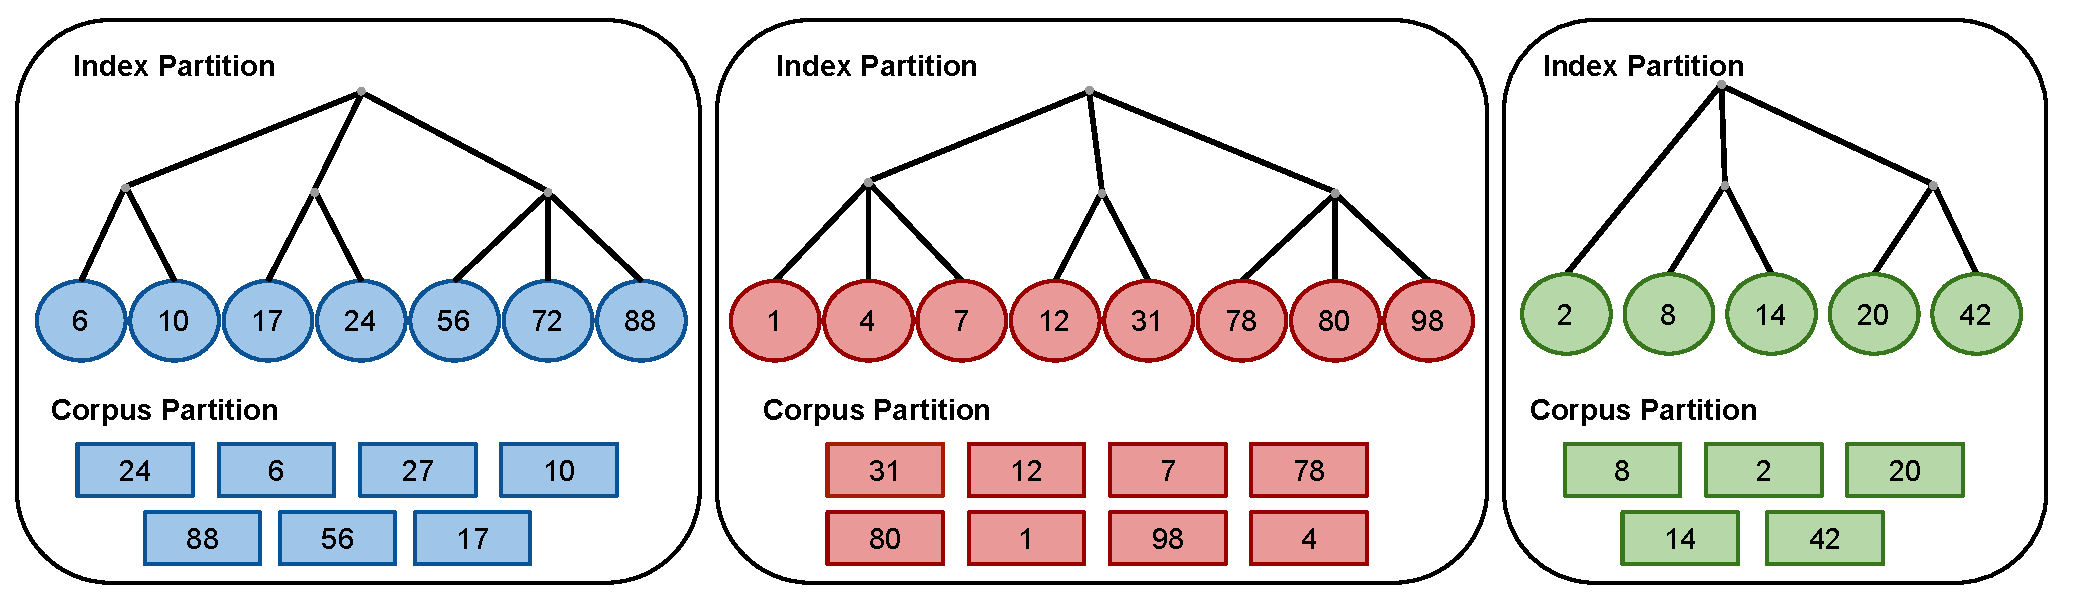
\includegraphics[width=\textwidth]{./figures/background/index_partitioning_by_doc.pdf}
        \caption{Index partitioning by document.}
        \label{fig:index_partitioning_by_doc}
    \end{minipage}%
    \begin{minipage}{.5\textwidth}
        \centering
        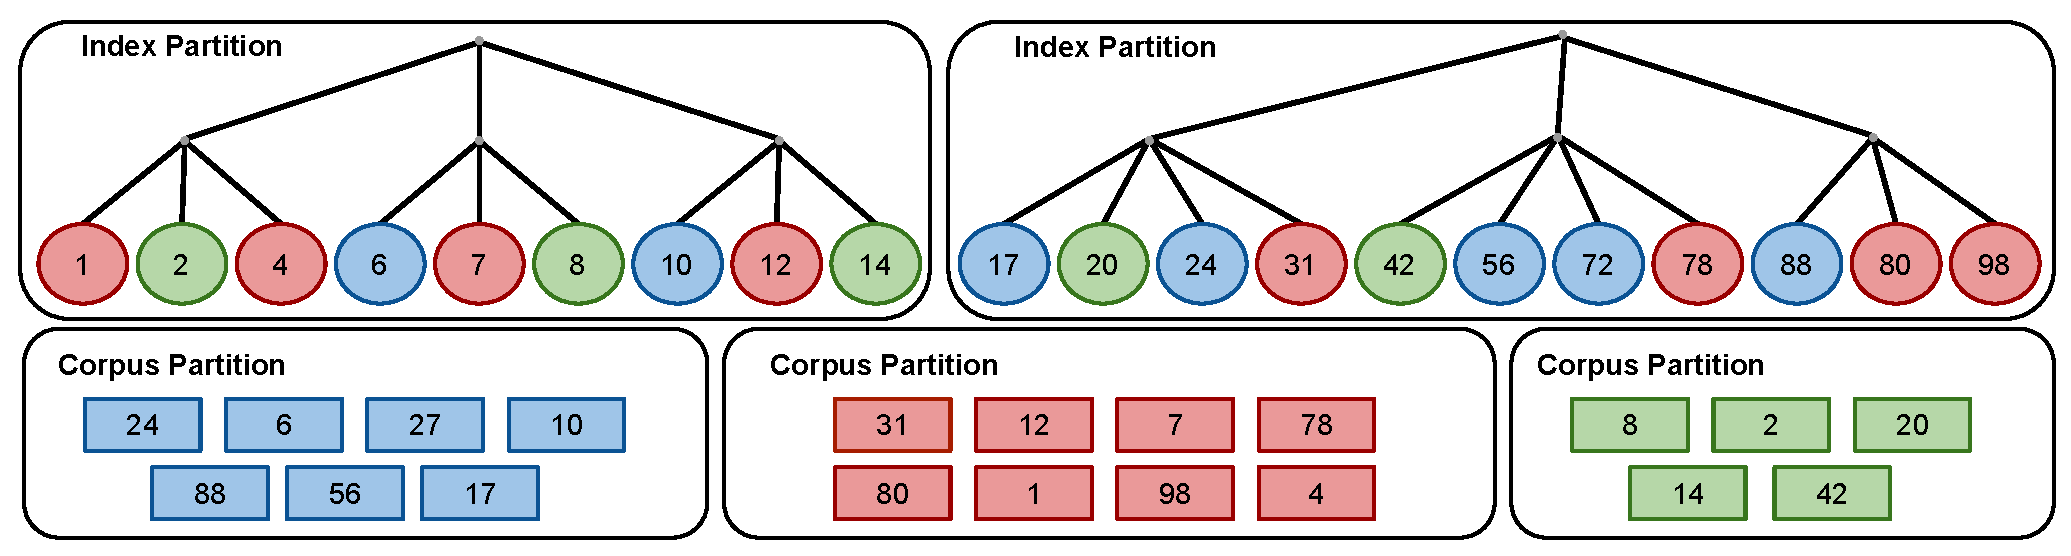
\includegraphics[width=\textwidth]{./figures/background/index_partitioning_by_term.pdf}
        \caption{Index partitioning by term.}
        \label{fig:index_partitioning_by_term}
    \end{minipage}
    \caption{Two approaches for partitioning a secondary index, given that the corpus table is partitioned by its primary key.
      In the partitioning by document approach the index is partitioned so that each index entry of a data item is co-located with the data item.
      In the partitioning by term approach the index partitioned so that each index partition contains index entries in a particular range.}
\end{figure}

\bigskip
\noindent
\textbf{Partitioning Secondary Indexes by Term.}
An alternative approach is to construct a logical ``global'' index that covers data in all partitions.
A global index, however, needs to be partitioned itself, as storing it on one node would likely become a bottleneck.

To partition a global index, the indexed terms can be used as the partition key (thus the term \textit{term-partitioned}
index).
Same as in base data partitioning, the index partitioning scheme can use the terms themselves, which can be useful for
range scans, or a the terms' hashes, which results to a more even load distribution.

The advantage of a term-partitioned index is that it can make reads more efficient:
rather than requiring a scatter/gather over all partitions, a lookup for a given term only needs to make a request to the
partition containing that term.
The downside of this approach is that writes are more complicated and slower:
a write to a single document may affect multiple partitions as the corresponding terms may correspond to multiple
different partitions.

HBase \cite{hbase:secondaryindexes} uses this approach:
Secondary indexes are stored in regular HBase tables, using the indexed attribute as primary key.
Term-partitioned indexes have also been used in the research systems such as SLIK \cite{kejriwal:slik}
and Diff-Index \cite{tan:diffindex}.

An index partitioned using this approach are commonly referred to as a \textit{global index}.

\medskip
\noindent
DynamoDB \cite{dynamodb:secondaryindexes} and Apache Phoenix \cite{phoenix:secondaryidnexing} support both local and global secondary indexes.

\subsubsection{Query Planning and Execution}

Most non-relational databases have simple query models that do not support complex operations such as aggregation and
joins.
However, some document-oriented databases like MongoDB \cite{mongodb:joins}, RethinkDB \cite{rethinkdb:joins},
and CouchDB \cite{couchdb:joins} support join operations.
Query planning in NoSQL databases mainly deals with the database's distribution model:
a query execution plans consist of routing query requests to the appropriate data or index partitions.


\section{Conclusion}
This chapter presented an overview of concepts related to query processing.
In particular, it presented query execution in relation database systems,
focusing on the implementation of query execution engines.
Furthermore, it described techniques used for improving query processing time,
including materialized views, caching, and secondary indexing.
The concepts presented in this chapter form the basis upon which the contributions of this thesis are built.